\documentclass[tikz,border=8pt]{standalone}
% Requer xelatex e a fonte Poppins. Ajuste o Path abaixo (ou use \setmainfont{Poppins} se ela estiver instalada).
\usepackage{fontspec}
\setmainfont{Poppins}[Path=/usr/share/fonts/truetype/google-fonts/,Extension=.ttf,UprightFont=*-Regular,BoldFont=*-Bold,ItalicFont=*-Italic,BoldItalicFont=*-BoldItalic]
\usepackage{xcolor}
\definecolor{azulescuro}{HTML}{4A6F9C}
\definecolor{azulmedio}{HTML}{6F93BC}
\definecolor{azulclaro}{HTML}{E9EDF3}
\definecolor{azulsenac}{HTML}{1F4E9A}
\definecolor{laranja}{HTML}{F19E37}
\definecolor{laranjaescuro}{HTML}{D9731A}
\definecolor{laranjaclaro}{HTML}{FDEFD9}
\definecolor{cinzatitulo}{HTML}{333333}
\definecolor{cinzatexto}{HTML}{5C5C5C}
\usepackage{tikz}
\usetikzlibrary{positioning,arrows.meta,fit,backgrounds,calc}

\definecolor{cinzabloco}{HTML}{E4E4E4}
\begin{document}
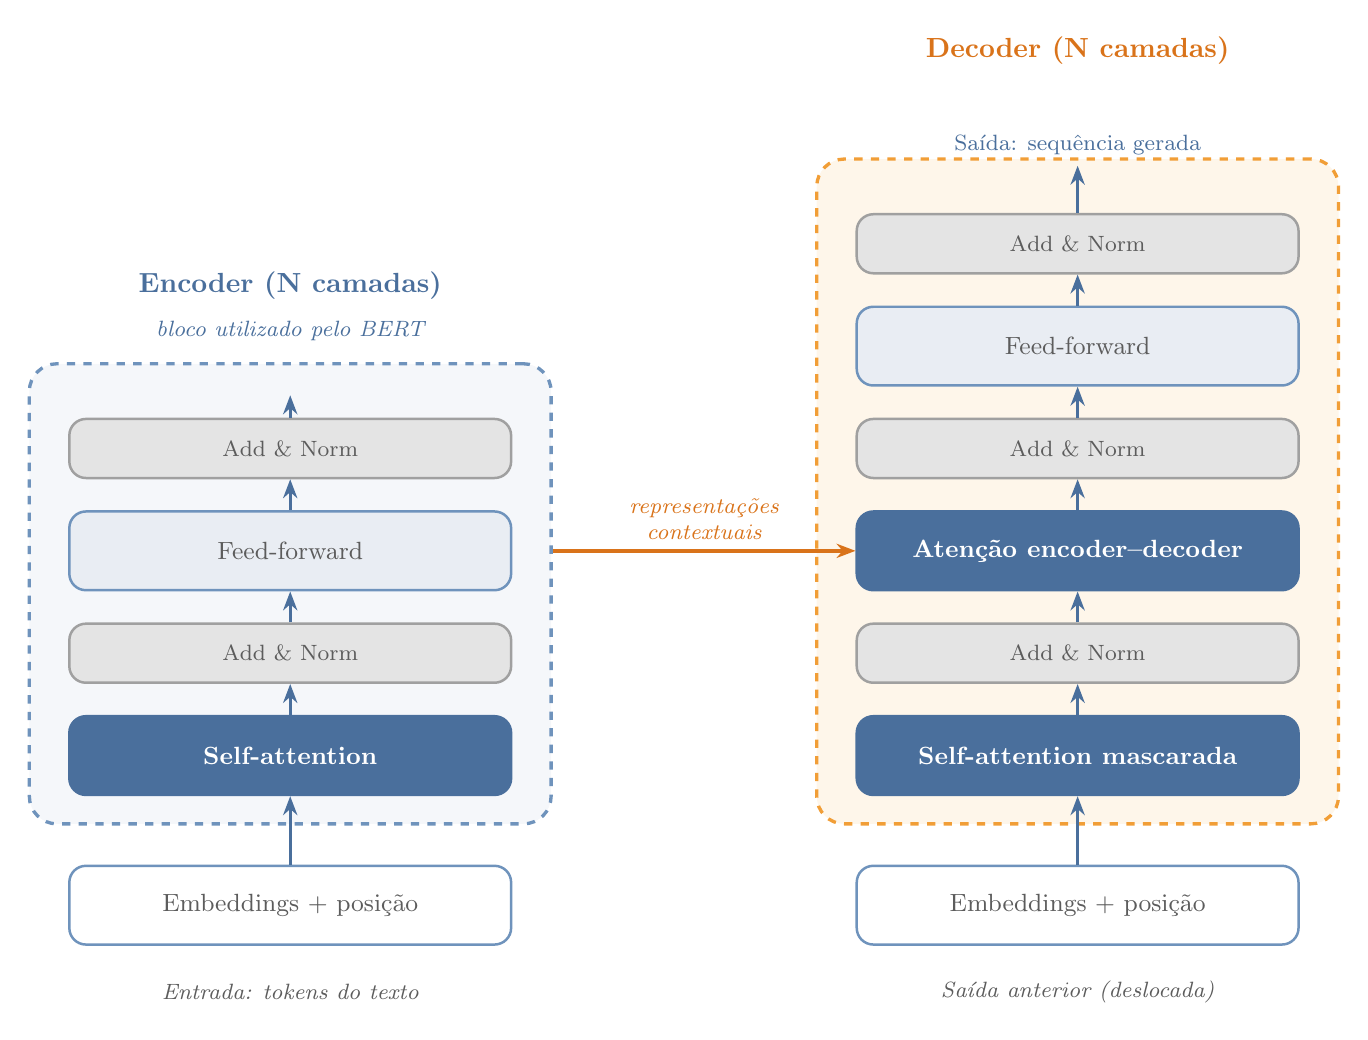
\begin{tikzpicture}[
    font=\small\color{cinzatexto},
    blk/.style={draw=azulmedio, fill=azulclaro, line width=0.9pt, rounded corners=6pt, align=center, minimum height=1.0cm, text width=5.4cm, inner sep=3pt},
    att/.style={blk, fill=azulescuro, draw=azulescuro, text=white, font=\small\bfseries},
    ffn/.style={blk},
    nrm/.style={blk, fill=cinzabloco, draw=cinzabloco!70!black, minimum height=0.75cm, font=\footnotesize, text=cinzatexto},
    emb/.style={blk, fill=white},
    seta/.style={-{Stealth[length=2.4mm]}, line width=1.2pt, color=azulescuro},
    rot/.style={font=\footnotesize\itshape\color{cinzatexto}, align=center}
]
% ---------- ENCODER (x=0)
\node[emb] (e0) at (0,0) {Embeddings + posição};
\node[att] (e1) at (0,1.9) {Self-attention};
\node[nrm] (e2) at (0,3.2) {Add \& Norm};
\node[ffn] (e3) at (0,4.5) {Feed-forward};
\node[nrm] (e4) at (0,5.8) {Add \& Norm};
\node[inner sep=0pt] (etop) at (0,6.5) {};
% ---------- DECODER (x=8.2)
\def\xd{10}
\node[emb] (d0) at (\xd,0) {Embeddings + posição};
\node[att] (d1) at (\xd,1.9) {Self-attention mascarada};
\node[nrm] (d2) at (\xd,3.2) {Add \& Norm};
\node[att] (d3) at (\xd,4.5) {Atenção encoder–decoder};
\node[nrm] (d4) at (\xd,5.8) {Add \& Norm};
\node[ffn] (d5) at (\xd,7.1) {Feed-forward};
\node[nrm] (d6) at (\xd,8.4) {Add \& Norm};
\node[inner sep=0pt] (dtop) at (\xd,9.1) {};
% ---------- molduras
\begin{scope}[on background layer]
\node[draw=azulmedio, dashed, line width=1.2pt, rounded corners=10pt, fill=azulclaro!45, fit=(e1)(e4)(etop), inner xsep=14pt, inner ysep=10pt] (enc) {};
\node[draw=laranja, dashed, line width=1.2pt, rounded corners=10pt, fill=laranjaclaro!55, fit=(d1)(d6)(dtop), inner xsep=14pt, inner ysep=10pt] (dec) {};
\end{scope}
\node[font=\footnotesize\itshape\color{azulescuro}, above=4pt of enc.north] (es) {bloco utilizado pelo BERT};
\node[font=\normalsize\bfseries\color{azulescuro}, above=1pt of es.north] {Encoder (N camadas)};
\node[font=\normalsize\bfseries\color{laranjaescuro}, above=30pt of dec.north] {Decoder (N camadas)};
% ---------- setas
\foreach \a/\b in {e0/e1,e1/e2,e2/e3,e3/e4,d0/d1,d1/d2,d2/d3,d3/d4,d4/d5,d5/d6}{\draw[seta] (\a) -- (\b);}
\draw[seta] (e4.north) -- (etop);
\draw[seta] (d6.north) -- ++(0,0.6) node[above, font=\footnotesize\color{cinzatexto}] {Saída: sequência gerada};
\draw[seta, color=laranjaescuro] (enc.east |- d3) -- node[above, rot] {representações\\contextuais} (d3.west);
% ---------- legendas inferiores
\node[rot] at (0,-1.1) {Entrada: tokens do texto};
\node[rot] at (\xd,-1.1) {Saída anterior (deslocada)};
\end{tikzpicture}
\end{document}
